\chapter{IONOSFERA}

A ionosfera é uma região ionizada da alta atmosfera, estendendo-se de 60 até 1000 km de altitude, assim, englobando partes da mesosfera, termosfera, e exosfera. Esta camada constitui-se de íons e elétrons livres criados primariamente por processo de fotoionização, e gás neutro. A fotoionização ionosférica consiste de um processo físico-químico, onde algumas espécies químicas presentes na atmosfera ganham ou perdem elétrons decorrentes da absorção de radiação solar predominantemente nas faixas ultravioleta, extremo ultravioleta e raios-X \cite{RISNBETH:1969, NEGRETI:2012}. A ionização, também, pode ocorrer devido a colisões com partículas altamente energéticas, provindas do meio solar ou galácticas, o que é mais facilmente observado em altas latitudes em fenômenos como auroral boreal.

A composição da ionosfera, assim, como a densidade do gases variam em função da altitude. A densidade de elétrons livres também varia, pois conforme a radiação penetra na atmosfera mais densa, a produção de elétrons aumenta até atingir um valor de pico em uma dada altitude. Abaixo desta, mesmo havendo um aumento na densidade da atmosfera neutra, a produção de elétrons decresce, pois a maior parte da radiação ionizante foi absorvida ao longo do percurso, e a taxa de recombinação predomina sobre a taxa de produção de elétrons. Devido as diferenças marcantes em termos de processos físicos e químicos que governam o comportamento da ionosfera, a mesma, pode ser dividida em camadas, onde cada uma apresenta um processo predominante. Finalmente, devido as drásticas mudanças em quantidade de radiação absorvida devido a transição entre noite e dia, existirão camadas que aparecem em um dado periódo.

A camada D é a mais interna, estando entre 60 e 90 km acima da superfície da Terra. Apresenta móleculas ionizadas de $NO$, $N_2$ e $O_2$. E, tem a maior razão de recombinação. Apresenta uma taxa de absorção considerável para ondas de radio de baixas e médias frequências, principalmente, devido a absorção de energia pelo elétrons livres, o que aumenta suas chances de colisão. Este efeito desaparece durante à noite, devido a uma menor ionização. Pode apresentar valores elevados de ionização em altas latitudes em decorrência de erupções solares com grandes quantidades de matéria hadrônica, prótons, em sua maioria, com uma duração de 24 à 48 horas.

A camada E é intermediária e está situada entre 90 e 150 km acima da superfície da Terra. A ionização decorre principalmente devido ao espalhamento de raio-X leve e ultravioleta distante (UV) provindos do Sol em moléculas de oxigênio. A estrutura vertical da camada E é determinada em sua maior parte pela competição entre efeitos de ionização e de recombinação. É importante pela presença de correntes elétricas que nela fluem e interagem com o campo magnético \cite{KIRCHHOFF:1991}. A noite, a camada E quase desaparece, pois sua fonte primaria de ionização não está presente.

A camada F se estende de 150 a mais de 500 km acima da superfície da Terra. Apresenta a maior concentração de elétrons, portanto, sinais que são capazes de penetrar até esta subcamada são capazes de escapar para o espaço. Predominam, nesta, a ionização de átomos de oxigênio por meio de radiação solar no espectro do extremo ultravioleta. A camada é subdivida em duas regiões, a F2 que está presente durante o dia e a noite, e a F1 que aparece somente durante o dia. 

A subcamada F2 engloba toda a região superior da ionosfera, inclusive a região de pico da densidade de elétrons. Este máximo no perfil vertical de ionização decorre do balanço entre os processos de transporte de plasma e os processos físico-químicos. Acima deste pico, a ionosfera se encontra em equilíbrio difusivo, ou seja, o plasma se distribui com a sua própria escala de altura. A presença do campo magnético contribui para a distribuição da ionização. A Figura \ref{fig:diagrama} apresenta as camadas D, E, F, assim como sua localização em relação à termosfera e magnetosfera.

\begin{figure}[h]
\center
\makebox[\textwidth][c]{
\subfigure[fig:ch11][Perfis verticais padronizados dos principais constituintes ionosféricos existentes acima de 90 km: $O_2^+$, $N_2^+$, $O^+$, $H^+$ e $N^+$. FONTE: Adaptado de Blelly e Alcaydé, \cite{KAMIDE:2007}]{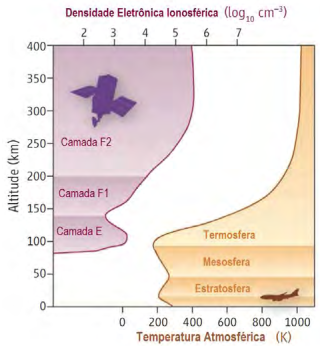
\includegraphics[width=9.5cm]{./Figuras/densidade_eletronica.png}}
\,\,
\subfigure[fig:ch12][Perfil de densidade ionosférica (curva à esquerda) e perfil de temperatura atmosférica (curva à direita). A Figura também mostra altitudes tipicas de vôos de aeronaves e órbitas baixas de satélites. FONTE: Adaptado de \cite{LASTOVICKA:2006}]{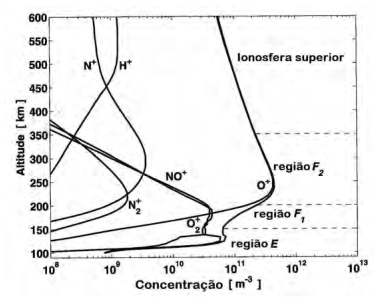
\includegraphics[width=9.5cm]{./Figuras/ionosfera_camadas.png}}
}
\caption{Diagramas apresentando a estrutura da ionosfera.}\label{fig:diagrama}
\end{figure}

\section{Regiões e Índices}

\subsection{Termosfera}

A termosfera se inicia aproximadamente a 90 km de altitude e não apresenta um limite superior bem definido, mas este deve estar entre 500 e 600 km de altitude. Nesta surgem os fenômenos de aurora, e nela também estão localizadas as órbitas da estação espacial, do ônibus espacial, assim como de vários satélites. Sua sua extensão, como as demais camadas da atmosfera, varia conforme a latitude. 

Temperatura é uma variável termodinâmica calculada como a média da energia cinética das moléculas, ou átomos, que compõem o sistema físico em questão. A temperatura na termosfera pode alcançar valores superiores a 2000 graus Celsius, entretanto, esta não pode ser medida por instrumentos convencionais, como por exemplo um termômetro, pois esta região é muito rarefeita, o que dificulta a transferência de energia térmica para o instrumento e, assim, sua quantificação. Assim, a temperatura é determinada por dados de satélites que alimentam expressões matemáticas baseadas em sua definição. Em geral, os altos valores se devem a grande taxa de absorção de radiação solar pelo nitrogênio e o oxigênio.

Assim como as demais camadas da atmosfera, também, sofre de processos convectivos que combinado com efeitos de gravidade e diferenças de pressão levam a formação de correntes, marés, análoga a dinâmica de outros fluidos como o oceano.

A ionosfera esta majoritariamente situada na termosfera, logo sua dinâmica esta diretamente acoplada a esta.

\subsection{Magnetosfera}

A magnetosfera é uma região delimitada pelo campo geomagnético. Pode ser tratada como um envoltório, recobrindo a Terra, e constitui a parte exterior da ionosfera, onde neste, a eletrodinâmica dos processos do plasma é dada pelo acoplamento com o campo magnético.

Por ser uma região mais externa tem interação direta com os ventos solares, o que leva  a uma distribuição não regular, pois a região voltada diretamente ao Sol sofre um processo de compressão, devido a pressão de radiação, enquanto no lado oposto existe a formação de uma estrutura análoga a um arrasto.

Em consequência de sua importante contribuição para a dinâmica ionosférica é interessante tratar e avaliar variáveis que forneçam informação sobre seu estado, como por exemplo, o Dst (Disturbance Storm Time) e o Kp (índice planetário).

\subsection{Índices Magnéticos}

O {\bf índice Dst} é uma medida da atividade geomagnética, geralmente utilizada para quantificar a intensidade de uma tempestade magnética. Apresenta resolução temporal de uma hora, e sua unidade de medida é o nanotesla (nT). É baseada no valor médio da componente horizontal do campo magnético, em quatro observatórios próximos ao equador magnético.

Em termos do índice Dst, pode-se considerar valores inferiores -30 nT como situações magnéticamente perturbadas. Os valores podem ser mapeados frente ao nível de pertubação da seguinte maneira, \cite{GONZALEZ:1994}: entre -30 nT e -50 nT tempestade geomagnética fraca; entre -50 nT -100 nT tempestade moderada; entre -100 nT e -250 nT tempestades muito intensas; abaixo de -250 nT supertempestades.

O {\bf índice Sym-H} descreve distúrbios no campo geomagnético em médias latitudes em termos de pertubações simétricas horizontais as linhas de campo magnético. Essencialmente é o mesmo que o índice DST, entretanto, apresenta uma resolução temporal de um minuto. Sua medida é realizada por um conjunto de seis estações em um sistema de coordenadas ligeiramente diferente. As estações que medem o Dst são diferentes daquelas que medem o Sym-H.

No trabalho \cite{WANLISS:2006} foi mostrado que os índices DST e Sym-H são equivalentes, em diversas configurações geomagnéticas, confirmando que o Sym-H poderia ser utilizado como uma alternativa de alta resolução temporal ao Dst.

O {\bf índice Kp} avalia as pertubações nas componentes horizontais do campo geomagnético global, e é baseado em medidas realizadas a cada 3 horas por magnetrômetros distribuídos ao redor do globo. Cada estação é calibrada segundo sua localização e reporta uma quantidade denominada de índice K dependendo da atividade geomagnética medida no local. Este é uma medida quase-logaritmica com resolução temporal de três horas de atividade geomagnética local com base em comparação com dias calmos. Cada estação mede o desvio máximo da componente horizontal. O índice Kp é gerado por uma combinação dos índices K e seu valor varia de 0 a 9 em intervalos discretos. 0 indica baixa atividade, enquanto 9 indica tempestades extremas, finalmente, fica associado os valores de 0 à 4 a períodos calmos, enquanto valores acima de 5 indicam tempestades magnéticas.

O {\bf índice ap}, que será utilizada neste trabalho, é semelhante ao índice Kp, e corresponde a uma transformação desse para uma escala linear. Varia entre 0 e 400 e sua relação com o Kp é dado na Tabela \ref{tab:kptoap}.

\begin{table}[hhh]
\begin{tabular}{|c|c|c|c|c|c|c|c|c|c|c|c|c|c|c|} \hline
Kp & 0  & 0+ & 1- & 1  & 1+ & 2- & 2   & 2+  & 3-  & 3   & 3+  & 4-  & 4   & 4+  \\ \hline
ap & 0  & 2  & 3  & 4  & 5  & 6  & 7   & 9   & 12  & 15  & 18  & 22  & 27  & 32  \\ \hline
Kp & 5- & 5  & 5+ & 6- & 6  & 6+ & 7-  & 7   & 7+  & 8-  & 8   & 8+  & 9-  & 9   \\ \hline
ap & 39 & 48 & 56 & 67 & 80 & 94 & 111 & 132 & 154 & 179 & 207 & 236 & 300 & 400 \\ \hline
\end{tabular}
\caption{Tabela de conversão entre os valores de Kp e ap. Fonte: https://www.ngdc.noaa.gov/stp/GEOMAG/kp\_ap.html.}
\label{tab:kptoap}
\end{table}

\section{Acoplamentos no Sistema Magnetosfera-Ionosfera}

É conhecido da eletrodinâmica clássica que em materiais condutores campos eletroestáticos devem ser nulos. E, a presença de campo elétrico só é permitido sob a ação de forças dinâmicas. Agora, um material condutor pode ser modelado como uma nuvem de gás de elétrons, onde apenas os portadores de cargas negativas podem se movimentar.

Essa aproximação de condutor pode ser usada como um ponto de partida para descrever o comportamento de um plasma sob campos elétricos. Assim, como o condutor, o plasma também é parcialmente uma nuvem de elétrons, entretanto, também possui portadores de cargas positivos e elementos neutros capazes de se mover. Em sua configuração de equilíbrio, isto é, na ausência de forças externas o campo elétrico médio deve ser nulo, assim, uma aproximação de campo ${\bf E_p}=0$ no referencial das partículas é adequado. Esta é chamada de aproximação magneto-hidrodinâmica (MHD), \cite{ROEDERER:1979} 

A teoria da relatividade restrita em uma aproximação de baixas velocidades, fornece a maneira pela qual campos elétricos e magnéticos se transformam sobre mudança de referencial, em um processo, análogo a composição de velocidades da física newtoniana.

Assim, no plano de referência das partículas a velocidade do plasma é nula, pois a partícula se move juntamente com o referencial. Agora, considere um sistema de referência fixo em relação a Terra e os seguintes campos vetoriais definidos neste: ${\bf v_p}$ um vetor de velocidade associada ao plasma, ${\bf B}$ um vetor de campo magnético e ${\bf E}$ um vetor de campo elétrico, fica valido a expressão

\begin{equation}
{\bf E_p}= {\bf E}+{\bf v_p}\times{\bf B}\mbox{.}
\end{equation}

Assim, um campo elétrico fica relacionado à velocidade do plasma e ao campo magnético por

\begin{equation}\label{eq:evb}
{\bf E}=-{\bf v_p}\times{\bf B}\mbox{.}
\end{equation}

A expressão \eqref{eq:evb} permite concluir a seguinte informação: um campo elétrico ${\bf E}$ perpendicular a ${\bf v_p}$ e ${\bf B}$ é gerado por partículas se movendo em um campo magnético. Finalmente, a componente de velocidade perpendicular a ${\bf B}$ se relaciona com ${\bf B}$ e ${\bf E}$ por

\begin{equation}\label{eq:veb}
{\bf v_d}=\frac{{\bf E}\times{\bf B}}{|{\bf B}|^2}\mbox{,}~
\end{equation}

onde ${\bf v_d}$ é a velocidade de deriva do plasma. As equações \eqref{eq:evb} e \eqref{eq:veb} expressam o mesmo fato, campo elétrico e velocidade estão conectados e um pode gerar o outro.

Alguns dos principais resultados destas relações, em aeronomia, é que estas servem como pedra angular para o desenvolvimento da teoria do dínamo ionosférico. Variações no campo geomagnético já eram conhecidas a mais de 300 anos, e a primeira causa proposta foi a presença de correntes elétricas fluindo na alta atmosfera. A necessidade da presença de portadores de carga para esta corrente levou a concepção do processo de ionização, e logo à existência da ionosfera.

Somente por volta de 1940 com a introdução da teoria do dínamo por Chapman E Bartels ficou bem elucidado o processo de formação das correntes na ionosfera. Segundo este modelo, ventos de marés produzem o movimento necessário das partículas carregadas. Em configurações fracamente excitadas, estes ventos podem ser divididos em duas componentes, uma com origem em variações solares, e a outra nas variações lunares. Isto permitiu pela a primeira vez o cálculo dos valores das correntes e suas magnitudes.

Os ventos de marés devido ao Sol são mais intensos, e são causados em sua maior parte por aquecimento, assim a contribuição gravitacional é menos intensa. Como resultado do movimento de marés e da viscosidade, os elétrons e os íons são arrastados através das linhas de campo magnético gerando campos elétricos, este fenômeno é o efeito dínamo.

Os campos elétricos do dínamo da região E tem sua origem nos ventos de marés associados a radiação solar ultravioleta absorvida na camada de ozônio, ao vapor de água na atmosfera, e efeitos gravitacionais gerados pela Lua. Em contra partida, o dínamo da região F tem sua origem nos ventos de marés térmicos que decorrem da absorção do radiação ultravioleta no extremo do espectro pela termosfera, \cite{ABDU:2005}.

A magnitude dos campos gerados pelo efeito dínamo esta diretamente acoplado a densidade de portadores de carga e, assim, as variações de iluminação ao longo do dia, variações do ciclo solar, com a longitude e latitude e com as estações do ano, por exemplo, \cite{FEJER:1999}.

\subsection{Dínamo da Região E} 

O dínamo da região E haje principalmente no lado diurno da Terra. O mecanismo de geração de correntes pode ser descrito de maneira simplista a partir da seguinte construção: seja ${\bf v}_m$ um campo vetorial de velocidade representativo do vento de maré, e ${\bf B}$ o campo geomagnético. O vento de maré desloca as partículas do plasma ao longo do campo magnético, aqui são observados três fenômenos: colisão entres portadores de cargas positivos, negativos e moléculas neutras, o processo de colisão transfere momento para as partículas carregadas o que gera uma corrente na direção leste; surgimento de movimentos em hélice devido ao acoplamento com o campo magnético; a separação de portadores com diferentes cargas e massas, o processo de transferência de momento por meio de colisão é dependente da massa, a separação entre as partículas gera um campo elétrico.

Assim, na região E os elétrons apresentam velocidades baixas, enquanto os íons serão transportados pelo vento. Logo, a separação de cargas induz um campo elétrico ${\bf E}$ dado por 

\begin{equation}
{\bf E_m} = {\bf v}_m\times{\bf B}\mbox{,}~
\end{equation}

o qual por sua vez induz uma corrente elétrica

\begin{equation}
{\bf J_m}=\sigma{\bf E_m} = \sigma{\bf v}_m\times{\bf B}\mbox{,}~
\end{equation}

onde $\sigma$ é a condutividade. O processo de separação de cargas deve também levar ao desenvolvimento de não homogeneidade na distribuição, isto é, acumulo de cargas, assim, a ionosfera sofre polarização. Finalmente, um campo elétrico de polarização é estabelecido e sua contribuição pode ser modelada em termos de um potencial elétrico, portanto, o campo elétrico total deve ser aproximadamente

\begin{equation}
{\bf E}_d = {\bf v}_m\times{\bf B}-{\bf \nabla}\phi\mbox{,}~
\end{equation}

onde $\phi$ é o potencial elétrico e ${\bf \nabla}\phi$ o campo elétrico devido a polarização. O sistema de correntes resultantes é dado por

\begin{equation}
{\bf J_d}=\tilde{\sigma}[{\bf v}_m\times{\bf B}-{\bf \nabla}\phi]\mbox{,}~
\end{equation}

onde $\tilde{\sigma}$ é o tensor de condutividade. A corrente associada ao dínamo da região E produz um movimento de deriva vertical (para cima) e zonal (para oeste) no período diurno.

\subsection{Dínamo da Região F}

Os ventos termosféricos na região F são horizontais e para oeste durante o dia. Isto provoca um movimento das partículas carregadas ao longo das linhas de campo magnético, proporcional a direção do vento na direção do campo. Existe também um movimento secundário com direção perpendicular tanto ao campo magnético quanto ao vento \cite{BATISTA:1986} dado por

\begin{equation}
{\bf v}=\frac{\nu\omega}{\nu^2+\omega^2}\frac{{\bf v_n}\times{\bf B}}{|{\bf B}|}\mbox{,}~
\end{equation}

onde ${\bf v}$ é a velocidade das partículas carregadas, ${\bf v_n}$ é a velocidade do vento neutro, ${\bf B}$ é o campo magnético, $\nu$ é a frequência de colisão entre partículas neutras e partículas neutras e $\omega={qB/m}$ é a girofrequência das partículas, sendo $q$ a carga e $m$ a massa.

Note a dependência com a carga na expressão da girofrequência, isto provoca uma distinção nos movimentos dos portadores de cargas positivos e negativos, ou seja, eles irão se separar, formando um campo elétrico de polarização. Durante o dia a região E pode ser modelada como um condutor que acoplado a região F leva a dispersão das cargas e restauração do equilíbrio; entretanto à noite este circuito não se fecha, pois a região E deixa de ser um condutor, e a formação do campo elétrico de polarização é possível.

As correntes do dínamo da região F são menos intensa do que as da região E, porém são de grande importância após o por do Sol. O campo elétrico de polarização da região F é vertical, e é o responsável pela intensificação da deriva vertical para cima ao anoitecer, o que é denominado de pico de pré-reversão.

\section{Anomalia de Ionização Equatorial}

As anomalias de interesse para este trabalho as bolhas de plasmas surgem de maneira acoplada a anomalia de ionização equatorial (AIE) que ocorre aproximadamente entre 15 e 20 graus de latitude magnética, tanto no hemisfério norte, quanto no hemisfério sul, na camada F2. A AIE consiste na formação de uma região de alta densidade eletrônica, e é uma anomalia, pois a densidade de plasma deveria ser maior em regiões equatoriais, e não em latitudes magnéticas mais altas.

Sua origem decorre da deriva vertical do plasma da camada F na região equatorial: os ventos termosféricos na camada F fazem surgir uma corrente elétrica apontando para leste, assim como um campo elétrico na mesma direção, enquanto o campo magnético aponta para o norte (lembrando que o dipolo magnético que modela o campo geomagnética da terra se encontra invertido, isto é, o norte magnético se situa no sul geográfico e o sul magnético se encontra no norte magnético), considerando então $\vec{E}\times\vec{B}$, tem-se o surgimento de uma força perpendicular ao campo magnético e ao campo elétrico, o que neste caso, aponta para cima, deslocando o plasmas para regiões de mais alta altitudes. Agora, quando em altas altitudes, o plasma for efeito gravitacional e diferença de pressão é trazido de volta à altitudes mais baixas, porém este movimento de descida é mais eficiente ao longo das linhas de campo magnético, levando a um aumento na densidade de plasma em regiões de médias latitudes.

\section{Bolhas de plasma}

Anomalias secundárias surgem durante o processo de formação da AIE quando considerado os demais acoplamentos como atração gravitacional, diferenças de pressões e processos de colisão. Em geral, estas apresentam um certo nível de organização devido às linhas de campo magnético da Terra. Isto ocorre pois partículas ionizadas ou carregas podem ser mover livremente ao longo das linhas magnéticas mas não entre elas.

Dentre as várias possíveis anomalias secundárias uma de particular interesse são as bolhas ionosféricas ou bolhas de plasma que podem ser definidas como regiões de baixa densidade de plasma ionosférico quando comparadas com a sua vizinhança. 

Em uma descrição grosseira pode-se dizer que surgem na região do equador magnético, após uma rápida elevação do plasma, devido a anomalia de ionização equatorial, isto é, o plasma ao acender cria regiões de baixa densidade.

pós sua formação podem evoluir para altas altitudes (centenas de quilômetros), estendendo-se ao longo das linhas de campo magnético (milhares de quilômetros) nas direções norte-sul, alcançado em torno de 20 graus de latitude magnética.


A cintilação ionosférica é uma variação rápida de amplitude e fase em sinais de radio frequência quando estes atravessam irregularidades no plasma ionosférico, como uma bolha de plasma, que é de particular interesse para este trabalho. Neste trabalho se realiza um estudo sobre algumas variáveis relacionadas com o efeito de cintilação ionosférica e com a estrutura de bolha no plasma.

\section{Variáveis para o estudo da cintilação ionosférica}

Existem várias quantidades que são necessárias para um estudo completo da dinâmica ionosférica como, por exemplo, medidas do fluxo de radiação solar, do campo magnético da Terra, da composição da atmosfera, nesta seção apresentar-se-á mais alguns destes índices.

O {\bf índice F10.7} é uma medida do fluxo solar na frequencia de 2800 MHz, ou em termos do comprimento de onda 10.7 cm. É um excelente indicador da atividade solar, uma vez que as emissões de rádio nesta frequencia se originam na alta cromosfera e nas regiões mais baixas da corona solar. Apresenta boa correlação com o número de manchas solares, assim como o número de irrandiância de ultravioleta e radiação solar visível. Tem um dos maiores históricos de dados coletados, iniciando em 1947. É reportada em unidades de fluxo solar (s.f.u), alcançado valores inferiores a 50 s.f.u e superiores a 300 s.f.u ao longo dos ciclos solares. Uma vez que a grande maioria da radiação ultravioleta que produz ionização na atmosfera terrestre tem origem na cromosfera solar, o índice F10.7 é um importante fator para avaliar a dinâmica da ionosfera.



O {\bf índice $S_4$} é utilizado para medir, avaliar, a cintilação ionosférica. Corresponde ao desvio padrão da intensidade do sinal de GPS de um minuto de dados, coletados com 50 amostras por segundo:

\begin{equation}
    S_4^2=\frac{\braket{I^2}-\braket{I}^2}{\braket{I}^2}\mbox{.}
\end{equation}
